\documentclass[tikz,border=2pt]{standalone}
\usepackage{tikz}
\usetikzlibrary{positioning}
\begin{document}
% Namikawa--Ueno type: I0-IV^*-t
% Target MRNC type: I0-IV^*-t
% Adapted from Tim Dokchitser picture: I_{g1}\e({\it n})IV^*
% Parameter substitution: n -> t
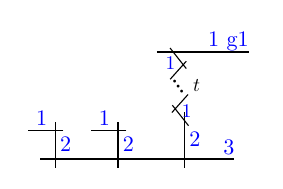
\begin{tikzpicture}[xscale=0.57,yscale=0.62]
\draw[thick,shorten >=2] (4/15,0)--(2263/480,0) node[inner sep=2pt,blue,above left,scale=0.8] {3};
\draw[shorten <=-3pt, shorten >=-3pt] (3/5,0)--node[inner sep=2pt,scale=0.8,blue,right] {2} (3/5,3/5);
\draw[shorten <=-3pt] (3/5,3/5)--node[inner sep=2pt,scale=0.8,blue,above] {1} (0,3/5);
\draw[shorten <=-3pt, shorten >=-3pt] (2,0)--node[inner sep=2pt,scale=0.8,blue,right] {2} (2,3/5);
\draw[shorten <=-3pt] (2,3/5)--node[inner sep=2pt,scale=0.8,blue,above] {1} (7/5,3/5);
\draw[shorten <=-3pt, shorten >=-3pt] (557/160,0)--node[inner sep=2pt,scale=0.8,blue,right] {2} (557/160,4/5);
\draw (557/160,4/5) 
    ++(0.09,-0.11)--++(-0.36,0.42)++(0.16,-0.15)  
    ++(0,0.02)
      node[blue,scale=0.7,inner sep=1,anchor=west]{1}
    ++(0,-0.02)
    ++(-0.17,0)--++(0.36,0.37)++(-0.14,0.04)  
    node{$\cdot$} ++(-0.08,0.1) node{$\cdot$}
    ++(-0.08,0.1) node{$\cdot$}++(0.19,-0.06)    node[auto,inner sep=5,scale=0.7,anchor=west]{$t$}
    ++(-0.29,0.13)--++(0.36,0.37)++(-0.19,0)   
    ++(0,-0.04)
      node[blue,scale=0.7,inner sep=1,anchor=east]{1}
    ++(0,0.04)
    ++(0.19,0)++(0,-0.15)--++(-0.36,0.42);
\draw[thick,shorten >=2] (43/15,353/160)--(151/30,353/160) node[inner sep=2pt,blue,above left,scale=0.8] {1 \smash{g}1};
\end{tikzpicture}
\end{document}
